\chapter{Avaliação de Desempenho}
\label{cap:avaliacao}

Este capítulo avalia empiricamente o desempenho da PolyglotImportCSV. A avaliação foi
listada como objetivo específico no Capítulo~\ref{cap:introducao} e apoia-se diretamente
no instrumento de medição descrito na seção~\ref{sec:observabilidade} --- o subsistema de
métricas, que cronometra cada fase da importação e registra o pico de memória por execução
--- e nos dois eixos de configuração descritos na seção~\ref{sec:execucao-estrategias}: a
estratégia de escrita (\texttt{naive} \textit{versus} \texttt{optimized}) e o modelo de
execução (\texttt{materialize} \textit{versus} \texttt{stream}). O objetivo não é eleger o
``melhor'' SGBD --- os cinco atendem a modelos de dados distintos --- mas caracterizar o
custo de importar um mesmo conjunto de dados para cinco paradigmas e quantificar o ganho
de cada uma das duas estratégias de desempenho da ferramenta.

A prática de comparar sistemas de dados sob uma carga sintética controlada e reproduzível
segue a tradição consolidada por \citeonline{cooper2010benchmarking} com o \textit{Yahoo!
Cloud Serving Benchmark} (YCSB), que estabeleceu o gerador de carga determinístico e as
métricas de \textit{throughput} como base para avaliar sistemas de dados heterogêneos. No
contexto específico de persistência poliglota, \citeonline{vanlanduyt2023comparative} e
\citeonline{ye2023benchmark} conduzem comparações de desempenho entre múltiplos modelos de
dados sob uma carga comum --- o mesmo princípio que orienta este capítulo, aqui aplicado à
etapa de \textbf{importação} e não à de consulta.

\section{Metodologia}
\label{sec:metodologia-avaliacao}

A avaliação é organizada em torno de seis \textbf{questões de pesquisa} (QP), que os
resultados da seção~\ref{sec:resultados} respondem:

\begin{itemize}
  \item \textbf{QP1 --- Custo por SGBD.} Qual é o \textit{throughput} de escrita de cada
        SGBD e como o tempo total de uma importação se decompõe entre as fases de leitura,
        seleção, mapeamento e escrita?
  \item \textbf{QP2 --- Modos de importação.} Importar a partir de um CSV por entidade
        (modo multifonte) ou de um único CSV combinado impõe sobrecustos distintos?
  \item \textbf{QP3 --- Escalabilidade.} Como o tempo e a memória evoluem ao multiplicar o
        volume de dados por dez, de mil a cem mil linhas?
  \item \textbf{QP4 --- Estratégia de escrita.} Qual é o ganho de desempenho da estratégia
        otimizada (vetorização e escrita em lote) sobre a ingênua (linha a linha)?
  \item \textbf{QP5 --- Modelo de execução.} Qual é o custo, em tempo e em pico de
        memória, do modo de fluxo em relação ao de materialização?
  \item \textbf{QP6 --- Memória limitada.} O pico de memória do modo de fluxo permanece
        constante em relação ao tamanho do arquivo, como prevê o seu projeto?
\end{itemize}

\subsection{Geração dos Dados}
\label{sec:geracao-dados}

A carga de trabalho é produzida por um \textbf{gerador determinístico} que sintetiza um
domínio de comércio eletrônico a partir de um único parâmetro de escala $N$ (o número de
produtos). As demais fontes crescem proporcionalmente a $N$: o estoque tem $N$ linhas, as
compras $3N$, as seleções $2N$ e os carrinhos $2N$. Todos os valores derivam de sementes
textuais fixas, de modo que a mesma escala $N$ produz \textbf{sempre os mesmos arquivos},
byte a byte, preservando a integridade referencial entre as fontes (todo produto
referenciado em uma compra existe no estoque). Essa reprodutibilidade é o que permite
comparar campanhas medidas em momentos diferentes: como a carga é idêntica, apenas o tempo
e a memória variam entre execuções. O uso de um gerador sintético parametrizável, em vez de
um conjunto de dados fixo, segue a mesma orientação metodológica do YCSB
\cite{cooper2010benchmarking}.

\subsection{Protocolo de Medição}
\label{sec:protocolo-medicao}

Cada célula experimental é definida por uma combinação de \textbf{tamanho} ($N \in \{1000,
10\,000, 100\,000\}$), \textbf{modo} (multifonte ou combinado), \textbf{estratégia}
(\texttt{naive} ou \texttt{optimized}), \textbf{modelo de execução} (\texttt{materialize}
ou \texttt{stream}) e é repetida \textbf{três vezes}. Antes de cada repetição, os cinco
SGBDs são \textbf{limpos} (\textit{cold-load}): as estruturas de destino são truncadas, de
modo que nenhuma repetição se beneficia de dados ou de caches deixados pela anterior. O
valor reportado para cada célula é a \textbf{mediana} das três repetições, que é robusta a
uma eventual repetição anômala.

O instrumento de medição impõe uma restrição metodológica importante. O tempo por fase é
cronometrado com um relógio de alta resolução; já o pico de memória é obtido instrumentando
as alocações do interpretador Python. Essa instrumentação de memória, porém, \textbf{infla
o tempo} das fases de leitura e mapeamento (cerca de $8{,}6\times$ a leitura e $6{,}5\times$
o mapeamento), enquanto quase não afeta a escrita nos bancos --- distorcendo, portanto, as
fases umas em relação às outras. Por isso, tempo e memória \textbf{não podem ser lidos da
mesma execução}. Adotou-se um \textbf{protocolo pareado}: duas campanhas idênticas em carga
e configuração, uma \textbf{com} a instrumentação de memória ativada (fonte dos picos de
memória) e outra \textbf{sem} ela (fonte dos tempos). As duas campanhas produziram
contagens de linhas idênticas em todas as células, confirmando que executam a mesma carga.
Ao longo do capítulo, \textbf{cada tabela e figura declara na legenda de qual das duas
campanhas os seus números provêm}, e valores de tempo e de memória nunca são combinados em
uma mesma linha.

Quanto à precisão, duas campanhas de tempo da mesma célula, sobre o mesmo código, chegaram
a diferir entre $15\%$ e $38\%$: as medidas de tempo carregam, portanto, uma incerteza da
ordem de $20\%$, e diferenças menores que isso não sustentam conclusões. O pico de memória,
ao contrário, reproduziu-se com diferença inferior a $0{,}1\%$ entre campanhas
independentes, sendo a métrica mais estável do estudo.

\section{Configuração Experimental}
\label{sec:config-experimental}

Todos os experimentos foram executados em uma \textbf{única máquina} com sistema
operacional Windows~11 (\textit{build} 10.0.26200) e Python 3.14.5. A semente global de
geração foi fixada em 42 e cada célula foi repetida três vezes. Os cinco SGBDs foram
providos por contêineres Docker, nas versões indicadas na
Tabela~\ref{tab:ambiente-sgbds}. Os contêineres partilham os recursos do mesmo hospedeiro
(8~GB de memória física); em particular, o Cassandra opera com um \textit{heap} de 1~GB
dentro de uma máquina virtual Docker de cerca de 3{,}8~GB --- uma restrição de ambiente que
se mostrará relevante na análise da fase de escrita.

\begin{table}[H]
  \caption{Imagens Docker dos SGBDs utilizadas na avaliação.}
  \label{tab:ambiente-sgbds}
  \centering
  \begin{tabular}{l l}
    \toprule
    \textbf{SGBD} & \textbf{Imagem Docker} \\
    \midrule
    PostgreSQL & \texttt{postgres:16-alpine} \\
    Redis      & \texttt{redis:7-alpine} \\
    MongoDB    & \texttt{mongo:7} \\
    Cassandra  & \texttt{cassandra:4.1} \\
    Neo4j      & \texttt{neo4j:5-community} \\
    \bottomrule
  \end{tabular}
  \par\vspace{4pt}
  {\footnotesize Fonte: Elaborado pelo autor (2026), a partir de \texttt{docker-compose.yml}.}
\end{table}

A matriz completa combina os três tamanhos, os dois modos, as duas estratégias e os dois
modelos de execução. Nem toda combinação é medida em todos os pontos: a estratégia
\texttt{naive} serve de linha de base e foi medida apenas no ponto $N = 10\,000$, no modo de
materialização, pois o modo de fluxo emprega sempre a via otimizada por projeto
(seção~\ref{sec:modelos-execucao}). Cada resultado a seguir indica o seu escopo.

\section{Resultados}
\label{sec:resultados}

\subsection{Estratégia de Escrita: Otimizada \textit{versus} Ingênua (QP4)}
\label{sec:res-estrategia}

A Tabela~\ref{tab:naive-optimized} contrasta as duas estratégias de escrita no ponto
$N = 10\,000$, no modo de materialização. A via otimizada importa o mesmo conjunto de dados
--- as mesmas \num{27494} linhas gravadas --- entre $8{,}5$ e $9{,}3$ vezes mais rápido que
a via ingênua. O ganho concentra-se, como esperado, nas duas fases que a otimização ataca:
o mapeamento (conversão de tipos), acelerado cerca de $42\times$ pela vetorização, e a
escrita, acelerada $7{,}7\times$ pela gravação em lote. A leitura e a seleção, que a
estratégia não altera, permanecem estáveis.

\begin{table}[H]
  \caption{Tempo total e das fases dominantes por estratégia de escrita, em segundos ($N = 10\,000$, materialização). Campanha sem instrumentação de memória.}
  \label{tab:naive-optimized}
  \centering
  \begin{tabular}{l r r r r r}
    \toprule
    \textbf{Modo} & \textbf{Estratégia} & \textbf{Mapeamento} & \textbf{Escrita} & \textbf{Total} & \textbf{Ganho} \\
    \midrule
    \multirow{2}{*}{multifonte} & ingênua   & 38{,}54 & 95{,}36 & 135{,}74 & --- \\
                                & otimizada &  0{,}91 & 12{,}44 &  14{,}54 & $9{,}3\times$ \\
    \midrule
    \multirow{2}{*}{combinado}  & ingênua   & ---     & ---     & 138{,}44 & --- \\
                                & otimizada & ---     & ---     &  16{,}30 & $8{,}5\times$ \\
    \bottomrule
  \end{tabular}
  \par\vspace{4pt}
  {\footnotesize Fonte: Elaborado pelo autor (2026), a partir de \texttt{benchmarks/timings-naive/}.}
\end{table}

\begin{figure}[H]
  \centering
  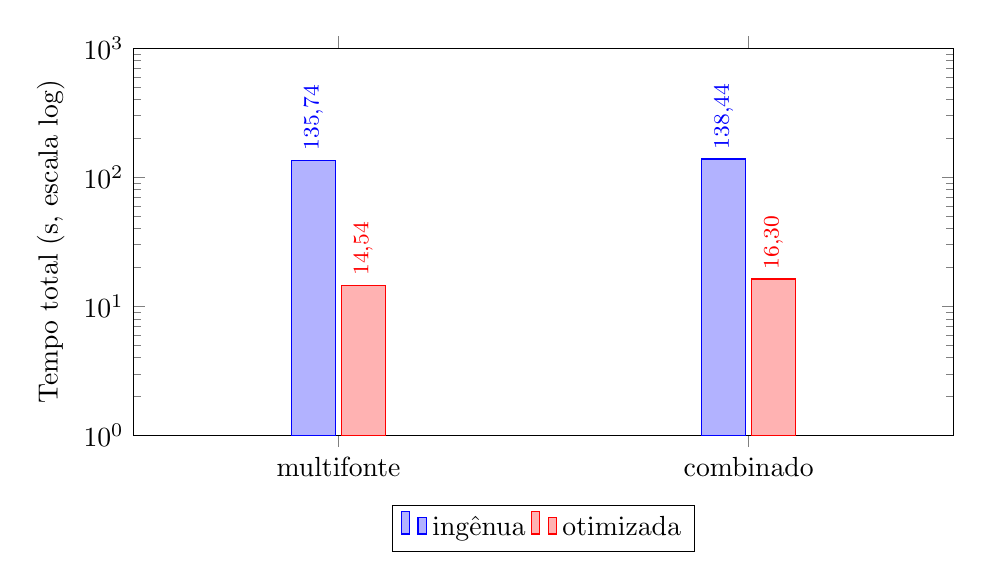
\begin{tikzpicture}
    \begin{axis}[
      ybar,
      width=12cm, height=6.5cm,
      ymode=log,
      log origin=infty,
      bar width=16pt,
      symbolic x coords={multifonte, combinado},
      xtick=data,
      ylabel={Tempo total (s, escala log)},
      ymin=1, ymax=1000,
      nodes near coords,
      point meta=explicit symbolic,
      nodes near coords style={font=\footnotesize, rotate=90, anchor=west},
      enlarge x limits=0.5,
      legend style={at={(0.5,-0.18)}, anchor=north, legend columns=-1},
      legend cell align=left,
    ]
      \addplot coordinates {(multifonte,135.74)[135,74] (combinado,138.44)[138,44]};
      \addplot coordinates {(multifonte,14.54)[14,54] (combinado,16.30)[16,30]};
      \legend{ingênua, otimizada}
    \end{axis}
  \end{tikzpicture}
  \caption{Tempo total de importação por estratégia de escrita ($N = 10\,000$, materialização; eixo vertical em escala logarítmica). Campanha sem instrumentação de memória.}
  \label{fig:naive-optimized}
  \par\vspace{4pt}
  {\footnotesize Fonte: Elaborado pelo autor (2026), a partir de \texttt{benchmarks/timings-naive/}.}
\end{figure}

Dado esse ganho, e por a estratégia otimizada ser o padrão da ferramenta, todos os demais
resultados deste capítulo empregam \texttt{optimized}. A estratégia ingênua cumpre aqui o
seu papel exclusivamente metodológico: a linha de base que dá sentido ao número
``$9{,}3\times$''.

\subsection{Decomposição por Fase e Escrita por SGBD (QP1)}
\label{sec:res-fases}

Fixada a estratégia otimizada, a Tabela~\ref{tab:fases-100k} decompõe uma importação de
$N = 100\,000$ linhas (multifonte, materialização) nas suas quatro fases. A escrita nos
bancos domina o custo, respondendo por cerca de $91\%$ do tempo total; a leitura e o
mapeamento, juntos, respondem por menos de $10\%$, e a seleção é desprezível.

\begin{table}[H]
  \caption{Tempo por fase de uma importação otimizada ($N = 100\,000$, multifonte, materialização), em segundos. Campanha sem instrumentação de memória.}
  \label{tab:fases-100k}
  \centering
  \begin{tabular}{l r r}
    \toprule
    \textbf{Fase} & \textbf{Tempo (s)} & \textbf{Participação} \\
    \midrule
    Leitura     &   7{,}69 & 5{,}1\% \\
    Seleção     &   0{,}00 & 0{,}0\% \\
    Mapeamento  &   5{,}90 & 3{,}9\% \\
    Escrita     & 136{,}34 & 91{,}0\% \\
    \midrule
    \textbf{Total} & 149{,}93 & 100\% \\
    \bottomrule
  \end{tabular}
  \par\vspace{4pt}
  {\footnotesize Fonte: Elaborado pelo autor (2026), a partir de \texttt{benchmarks/timings/}.}
\end{table}

Como a escrita concentra o custo, convém abri-la por SGBD. A
Tabela~\ref{tab:escrita-sgbd} e a Figura~\ref{fig:throughput-sgbd} apresentam, para a mesma
importação, o número de linhas gravadas, o tempo de escrita e o \textit{throughput}
resultante em cada um dos cinco bancos. Os valores variam por mais de uma ordem de
grandeza: o MongoDB grava a cerca de \num{14431}~linhas/s, enquanto o Cassandra fica em
$912$~linhas/s.

\begin{table}[H]
  \caption{Escrita por SGBD em uma importação otimizada ($N = 100\,000$, multifonte, materialização). Campanha sem instrumentação de memória.}
  \label{tab:escrita-sgbd}
  \centering
  \begin{tabular}{l r r r}
    \toprule
    \textbf{SGBD} & \textbf{Linhas} & \textbf{Tempo (s)} & \textbf{Linhas/s} \\
    \midrule
    Cassandra  & \num{100000} & 109{,}61 &   $912$ \\
    Neo4j      &  \num{51602} &  13{,}23 & \num{3901} \\
    PostgreSQL &  \num{62167} &   8{,}13 & \num{7644} \\
    Redis      &  \num{49558} &   4{,}56 & \num{10865} \\
    MongoDB    &  \num{11609} &   0{,}80 & \num{14431} \\
    \bottomrule
  \end{tabular}
  \par\vspace{4pt}
  {\footnotesize Fonte: Elaborado pelo autor (2026), a partir de \texttt{benchmarks/timings/}.}
\end{table}

\begin{figure}[H]
  \centering
  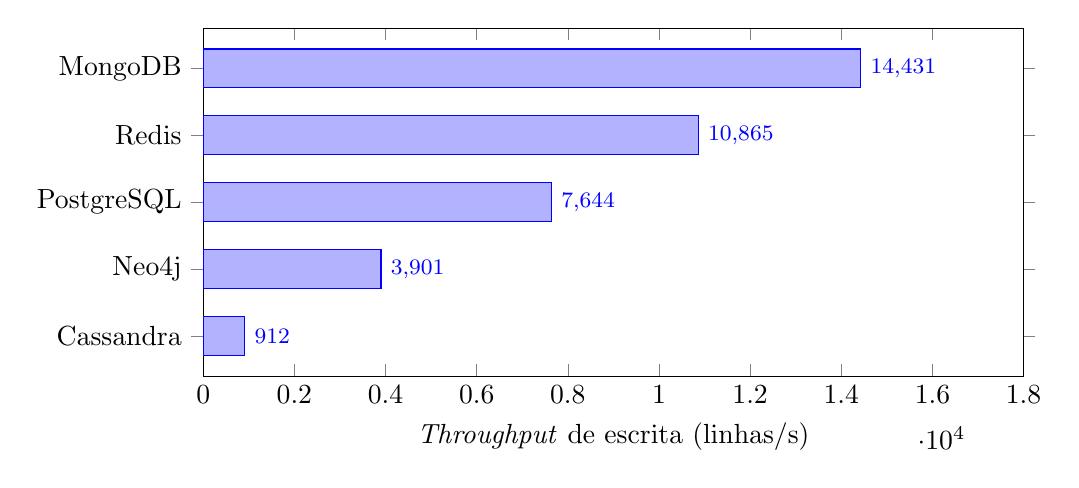
\begin{tikzpicture}
    \begin{axis}[
      xbar,
      width=12cm, height=6cm,
      bar width=14pt,
      symbolic y coords={Cassandra, Neo4j, PostgreSQL, Redis, MongoDB},
      ytick=data,
      xlabel={\textit{Throughput} de escrita (linhas/s)},
      xmin=0, xmax=18000,
      nodes near coords={\pgfmathprintnumber[fixed, precision=0]{\pgfplotspointmeta}},
      nodes near coords style={font=\footnotesize},
      enlarge y limits=0.15,
    ]
      \addplot coordinates {(912,Cassandra) (3901,Neo4j) (7644,PostgreSQL) (10865,Redis) (14431,MongoDB)};
    \end{axis}
  \end{tikzpicture}
  \caption{\textit{Throughput} de escrita por SGBD ($N = 100\,000$, multifonte, materialização, estratégia otimizada). Campanha sem instrumentação de memória.}
  \label{fig:throughput-sgbd}
  \par\vspace{4pt}
  {\footnotesize Fonte: Elaborado pelo autor (2026), a partir de \texttt{benchmarks/timings/}.}
\end{figure}

O Cassandra sozinho responde por $109{,}6$~s dos $136{,}3$~s da fase de escrita --- cerca de
$80\%$. Qualquer afirmação sobre ``o tempo de escrita'' é, portanto, em larga medida uma
afirmação sobre o Cassandra neste ambiente, o que reforça a necessidade de abrir a fase por
SGBD em vez de tratá-la como um bloco único.

\subsection{Modos de Importação: Multifonte \textit{versus} Combinado (QP2)}
\label{sec:res-modos}

Os dois modos de importação --- um CSV por entidade ou um único CSV combinado --- gravam os
mesmos dados e, como mostra a Tabela~\ref{tab:multi-combined}, têm desempenho muito próximo.
No ponto de $100\,000$ linhas, o modo combinado é cerca de $8\%$ mais lento em tempo e usa
cerca de $6\%$ mais memória --- diferenças da ordem da própria incerteza de medição do
tempo ($\approx 20\%$). Na prática, os dois modos são intercambiáveis em custo, e a escolha
entre eles é de conveniência de organização dos dados, não de desempenho.

\begin{table}[H]
  \caption{Multifonte \textit{versus} combinado ($N = 100\,000$, estratégia otimizada). Tempos e picos de memória provêm de campanhas distintas, conforme indicado.}
  \label{tab:multi-combined}
  \centering
  \begin{tabular}{l r r r r}
    \toprule
    & \multicolumn{2}{c}{\textbf{Materialização}} & \multicolumn{2}{c}{\textbf{Fluxo}} \\
    \cmidrule(lr){2-3} \cmidrule(lr){4-5}
    \textbf{Modo} & \textbf{Tempo (s)} & \textbf{Pico (MB)} & \textbf{Tempo (s)} & \textbf{Pico (MB)} \\
    \midrule
    multifonte & 149{,}93 &  950{,}7 & 165{,}03 & 75{,}9 \\
    combinado  & 161{,}94 & \num{1009.5} & 181{,}42 & 79{,}8 \\
    \bottomrule
  \end{tabular}
  \par\vspace{4pt}
  {\footnotesize Fonte: Elaborado pelo autor (2026). Tempo de \texttt{benchmarks/timings/}; memória de \texttt{benchmarks/}.}
\end{table}

\subsection{Modelos de Execução: Memória e Tempo (QP5 e QP6)}
\label{sec:res-execucao}

O resultado central da avaliação está no contraste entre materialização e fluxo. A
Tabela~\ref{tab:memoria} e a Figura~\ref{fig:memoria} mostram o pico de memória dos dois
modelos em função do tamanho do arquivo, no modo multifonte. A materialização cresce
\textbf{linearmente} com o volume: de $10{,}5$~MB em mil linhas para $950{,}7$~MB em cem mil
--- praticamente $90\times$ mais memória para $100\times$ mais dados. O fluxo, ao contrário,
\textbf{achata}: de $10{,}7$~MB para $75{,}9$~MB no mesmo intervalo. Em cem mil linhas, o
fluxo usa \textbf{$12{,}5\times$ menos memória} que a materialização, e a vantagem cresce
com o tamanho do arquivo. Esse achatamento é a evidência empírica que responde à QP6: o pico
do modo de fluxo é governado pelo tamanho do bloco, não pelo do arquivo, exatamente como
prevê o seu projeto (seção~\ref{sec:modelos-execucao}).

\begin{table}[H]
  \caption{Pico de memória por modelo de execução ($N$ crescente, multifonte, estratégia otimizada), em MB. Campanha com instrumentação de memória.}
  \label{tab:memoria}
  \centering
  \begin{tabular}{r r r r}
    \toprule
    \textbf{Linhas} & \textbf{Materialização} & \textbf{Fluxo} & \textbf{Razão} \\
    \midrule
    \num{1000}   &  10{,}5 & 10{,}7 & $0{,}98\times$ \\
    \num{10000}  &  95{,}3 & 47{,}8 & $2{,}0\times$ \\
    \num{100000} & 950{,}7 & 75{,}9 & $\mathbf{12{,}5\times}$ \\
    \bottomrule
  \end{tabular}
  \par\vspace{4pt}
  {\footnotesize Fonte: Elaborado pelo autor (2026), a partir de \texttt{benchmarks/} (raiz).}
\end{table}

\begin{figure}[H]
  \centering
  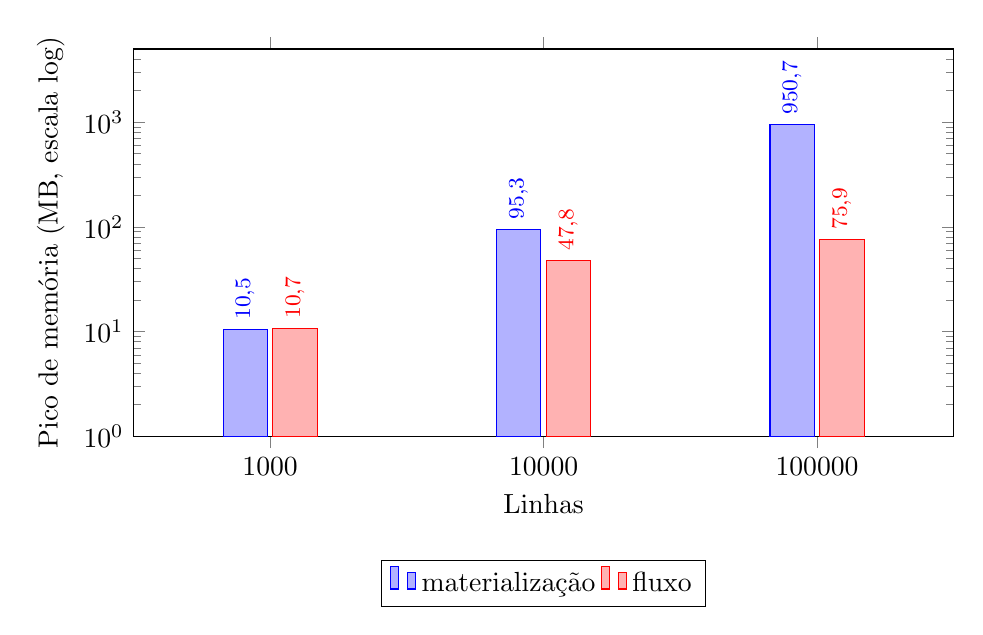
\begin{tikzpicture}
    \begin{axis}[
      ybar,
      width=12cm, height=6.5cm,
      ymode=log,
      log origin=infty,
      bar width=16pt,
      symbolic x coords={1000, 10000, 100000},
      xtick=data,
      xlabel={Linhas},
      ylabel={Pico de memória (MB, escala log)},
      ymin=1, ymax=5000,
      nodes near coords,
      point meta=explicit symbolic,
      nodes near coords style={font=\footnotesize, rotate=90, anchor=west},
      enlarge x limits=0.25,
      legend style={at={(0.5,-0.32)}, anchor=north, legend columns=-1},
      legend cell align=left,
    ]
      \addplot coordinates {(1000,10.5)[10,5] (10000,95.3)[95,3] (100000,950.7)[950,7]};
      \addplot coordinates {(1000,10.7)[10,7] (10000,47.8)[47,8] (100000,75.9)[75,9]};
      \legend{materialização, fluxo}
    \end{axis}
  \end{tikzpicture}
  \caption{Pico de memória por modelo de execução em função do volume (multifonte, escala logarítmica): a materialização cresce com o arquivo; o fluxo achata.}
  \label{fig:memoria}
  \par\vspace{4pt}
  {\footnotesize Fonte: Elaborado pelo autor (2026), a partir de \texttt{benchmarks/} (raiz).}
\end{figure}

Essa economia de memória tem um custo em tempo, mas modesto e \textbf{decrescente}. A
Tabela~\ref{tab:tempo-execucao} e a Figura~\ref{fig:tempo-execucao} mostram que o
sobrecusto de tempo do fluxo cai de $+61\%$ em mil linhas para apenas $+10\%$ em cem mil.
A razão é que, à medida que o volume cresce, a escrita nos bancos --- comum aos dois modelos
--- passa a dominar o tempo total, diluindo o custo fixo do processamento entrelaçado do
fluxo. Ou seja: \textbf{quanto maior o arquivo, mais barata fica a troca} --- a vantagem de
memória do fluxo cresce justamente onde o seu custo de tempo encolhe.

\begin{table}[H]
  \caption{Tempo total por modelo de execução ($N$ crescente, multifonte, estratégia otimizada), em segundos. Campanha sem instrumentação de memória.}
  \label{tab:tempo-execucao}
  \centering
  \begin{tabular}{r r r r}
    \toprule
    \textbf{Linhas} & \textbf{Materialização} & \textbf{Fluxo} & \textbf{Sobrecusto} \\
    \midrule
    \num{1000}   &   2{,}87 &   4{,}63 & $+61\%$ \\
    \num{10000}  &  16{,}20 &  20{,}94 & $+29\%$ \\
    \num{100000} & 149{,}93 & 165{,}03 & $+10\%$ \\
    \bottomrule
  \end{tabular}
  \par\vspace{4pt}
  {\footnotesize Fonte: Elaborado pelo autor (2026), a partir de \texttt{benchmarks/timings/}.}
\end{table}

\begin{figure}[H]
  \centering
  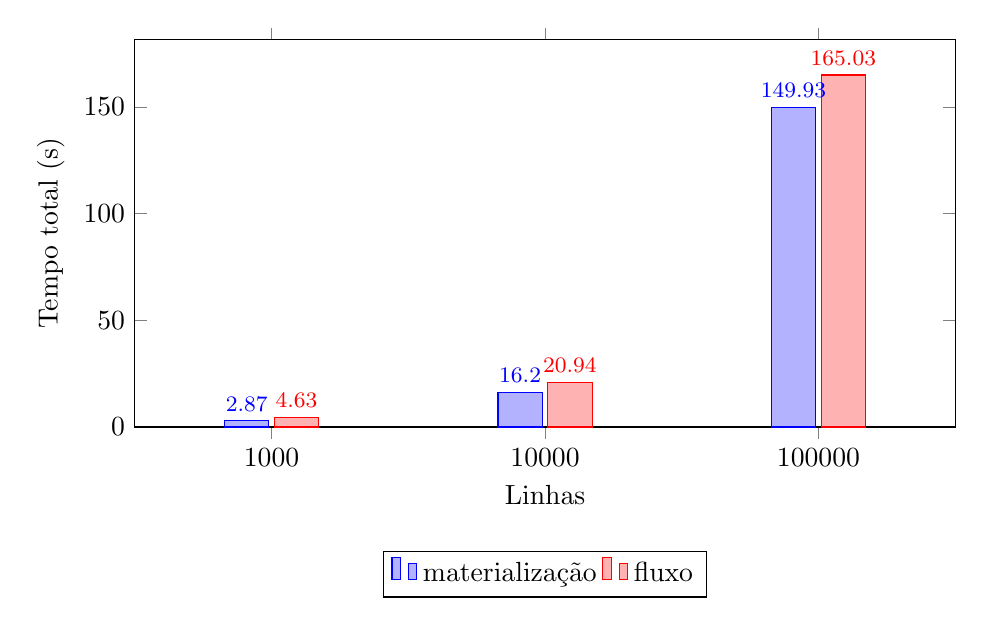
\begin{tikzpicture}
    \begin{axis}[
      ybar,
      width=12cm, height=6.5cm,
      bar width=16pt,
      symbolic x coords={1000, 10000, 100000},
      xtick=data,
      xlabel={Linhas},
      ylabel={Tempo total (s)},
      ymin=0,
      nodes near coords={\pgfmathprintnumber[fixed, precision=2]{\pgfplotspointmeta}},
      nodes near coords style={font=\footnotesize},
      enlarge x limits=0.25,
      legend style={at={(0.5,-0.32)}, anchor=north, legend columns=-1},
      legend cell align=left,
    ]
      \addplot coordinates {(1000,2.87) (10000,16.20) (100000,149.93)};
      \addplot coordinates {(1000,4.63) (10000,20.94) (100000,165.03)};
      \legend{materialização, fluxo}
    \end{axis}
  \end{tikzpicture}
  \caption{Tempo total por modelo de execução em função do volume (multifonte): o sobrecusto do fluxo encolhe de $+61\%$ para $+10\%$ à medida que a escrita passa a dominar.}
  \label{fig:tempo-execucao}
  \par\vspace{4pt}
  {\footnotesize Fonte: Elaborado pelo autor (2026), a partir de \texttt{benchmarks/timings/}.}
\end{figure}

\subsection{Uma Observação sobre o Pico de Memória da Estratégia Otimizada}
\label{sec:res-tradeoff}

Um ponto exige cuidado na leitura das medidas de memória. No mesmo ponto de $10\,000$ linhas
e modo de materialização, a estratégia \textbf{ingênua} exibe um pico \textbf{menor} que a
otimizada --- $14{,}4$~MB contra $95{,}4$~MB no modo multifonte
(Tabela~\ref{tab:tradeoff-memoria}). O número não é um erro, e reproduz-se entre campanhas.
A explicação está na natureza da otimização: para gravar em lote, o caminho otimizado
\textbf{acumula registros em memória} antes de despachá-los. No Neo4j, em particular, a
gravação de relacionamentos por \texttt{UNWIND} monta a lista completa de arestas de uma
entidade em memória antes de submetê-la, ao passo que a via ingênua percorre as arestas uma
a uma, sem acumular. A escrita em lote, portanto, \textbf{troca memória por vazão}: ela é
$7{,}7\times$ mais rápida (Tabela~\ref{tab:naive-optimized}), mas ao preço de um pico de
memória maior.

\begin{table}[H]
  \caption{Pico de memória por estratégia de escrita ($N = 10\,000$, materialização), em MB. Campanha com instrumentação de memória.}
  \label{tab:tradeoff-memoria}
  \centering
  \begin{tabular}{l r r}
    \toprule
    \textbf{Modo} & \textbf{Ingênua} & \textbf{Otimizada} \\
    \midrule
    multifonte & 14{,}4 & 95{,}4 \\
    combinado  & 21{,}3 & \num{101.6} \\
    \bottomrule
  \end{tabular}
  \par\vspace{4pt}
  {\footnotesize Fonte: Elaborado pelo autor (2026), a partir de \texttt{benchmarks/naive/}.}
\end{table}

Vale notar que esse acúmulo é justamente o que o \textbf{modo de fluxo} limita: ao processar
o arquivo em blocos, ele mantém em memória apenas um bloco e os lotes ainda não descarregados
--- e é por isso que o fluxo, mesmo empregando sempre a via otimizada, atinge picos muito
menores que a materialização otimizada (Tabela~\ref{tab:memoria}). Os dois eixos, portanto,
atuam sobre a memória de formas complementares.

\section{Análise e Discussão}
\label{sec:discussao-avaliacao}

Os resultados respondem às seis questões de pesquisa. A escrita nos bancos é a fase
dominante de uma importação (QP1): mais de $90\%$ do tempo em cem mil linhas, com
\textit{throughput} que varia por mais de uma ordem de grandeza entre SGBDs. Essa dispersão
reflete o modelo de dados de cada banco e a forma de gravação idiomática correspondente --- o
MongoDB e o Redis, orientados a inserções em massa simples, lideram; o Cassandra e o Neo4j,
que na configuração deste estudo aplicam respectivamente escrita replicada e \texttt{MERGE}
com verificação de unicidade, ficam atrás. Trata-se de uma manifestação, na etapa de
importação, das mesmas diferenças de paradigma que a literatura observa na etapa de consulta
\cite{muniswamaiah2023comparison, vanlanduyt2023comparative}.

Os dois modos de importação são equivalentes em custo (QP2), o que confirma, do ponto de
vista de desempenho, a equivalência de resultados entre eles já assegurada por teste
(seção~\ref{sec:modelos-execucao}). Quanto à escalabilidade (QP3), o tempo cresce de forma
aproximadamente proporcional ao volume, governado pela fase de escrita, enquanto a memória
segue o modelo de execução escolhido.

O maior ganho de engenharia está nos dois eixos de desempenho. A estratégia otimizada
acelera a importação em cerca de $9\times$ (QP4), pela vetorização da conversão de tipos e
pela escrita em lote. O modo de fluxo reduz o pico de memória em $12{,}5\times$ em cem mil
linhas (QP5), a um custo de tempo de apenas $+10\%$ nesse ponto --- e o achatamento do pico
com o volume (QP6) confirma que o fluxo importa com memória \textbf{constante} no tamanho do
arquivo. É esse último resultado que sustenta a principal afirmação de projeto da
ferramenta: a de importar arquivos maiores que a memória disponível, algo impossível no modo
de materialização.

\subsection{Ameaças à Validade}
\label{sec:ameacas-validade}

Os resultados devem ser lidos à luz de algumas limitações. Quanto à \textbf{validade de
construção}, os tempos carregam incerteza da ordem de $20\%$ (seção~\ref{sec:protocolo-medicao}),
de modo que diferenças menores que isso não foram interpretadas como significativas; o pico
de memória, muito mais estável ($0{,}1\%$), não sofre dessa limitação. A separação em
campanhas pareadas para tempo e memória evita a distorção que a instrumentação de memória
introduziria nas fases, mas impede a leitura das duas métricas de uma mesma execução.

Quanto à \textbf{validade externa}, todos os experimentos correram em uma única máquina, sob
Windows, com os cinco SGBDs em contêineres partilhando 8~GB de memória física. Esse ambiente
não representa uma implantação de produção, com bancos dedicados e ajustados. O caso mais
sensível é o do Cassandra, cujo \textit{throughput} de escrita ($912$~linhas/s) reflete um
\textit{heap} de 1~GB em uma máquina virtual apertada --- uma restrição de \textbf{ambiente},
não uma propriedade intrínseca do SGBD; um Cassandra provisionado adequadamente reduziria
substancialmente a sua parcela na fase de escrita. Quanto à \textbf{validade interna}, o
gerador determinístico e a limpeza dos bancos antes de cada repetição isolam o efeito
medido, mas o volume avaliado (até cem mil linhas) é moderado, e não se explorou o efeito de
caches quentes nem de execuções concorrentes. Aprofundar o caminho de escrita do Cassandra e
estender o estudo a volumes maiores figuram entre as atividades futuras
(Capítulo~\ref{cap:futuros}).
